\documentclass[11pt]{article}
\usepackage[T1]{fontenc}
\usepackage{lmodern}
\usepackage[margin=1in]{geometry}
\usepackage{microtype}
\usepackage{amsmath,amssymb,amsthm,mathtools}
\usepackage{tikz}
\usepackage[colorlinks=true,linkcolor=blue,citecolor=blue,urlcolor=blue]{hyperref}
\hypersetup{pdftitle={An Upper Bound of 9/4 for the Matrix Multiplication Exponent},pdfauthor={OpenAI}}
\newtheorem{theorem}{Theorem}[section]
\newtheorem{proposition}[theorem]{Proposition}
\newtheorem{lemma}[theorem]{Lemma}
\newtheorem{corollary}[theorem]{Corollary}
\theoremstyle{definition}
\newtheorem{definition}[theorem]{Definition}
\theoremstyle{remark}
\newtheorem{remark}[theorem]{Remark}
\DeclareMathOperator{\rank}{R}
\newcommand{\C}{\mathbb C}
\newcommand{\R}{\mathbb R}
\newcommand{\N}{\mathbb N}
\newcommand{\degen}{\mathrel{\rightsquigarrow}}
\newcommand{\eps}{\varepsilon}
\numberwithin{equation}{section}
\title{An Upper Bound of $9/4$ for the\\Matrix Multiplication Exponent}
\author{OpenAI}
\date{October 2, 2026}

\begin{document}
\maketitle

\begin{abstract}
We prove that the exponent of matrix multiplication over the complex
numbers is at most $9/4$.
\end{abstract}

\section{Introduction}\label{sec:intro}

The exponent $\omega$ of matrix multiplication over $\C$ is the infimum
of the real numbers $\tau$ such that, for every $\eps>0$, two $n\times n$
matrices can be multiplied in $O_\eps(n^{\tau+\eps})$ scalar arithmetic
operations. The dimension $n$ tends to infinity; the algorithm and its
constants may depend on $\eps$. We prove the following bound.

\begin{theorem}\label{thm:main}
For every $\eps>0$, two $n\times n$ complex matrices can be multiplied
using $O_\eps(n^{9/4+\eps})$ arithmetic operations. In particular,
$\omega\leq9/4$.
\end{theorem}

Strassen's seven-product algorithm for two-by-two matrices showed
that recursion can reduce the arithmetic exponent below
three~\cite{Str69}. Bilinear algorithms can be represented by
trilinear coefficient arrays, or tensors; linear substitutions and
tensor products then express reductions and recursive composition.
Approximate bilinear algorithms enlarge the available constructions,
and Bini's interpolation argument converts them into exact asymptotic
algorithms~\cite{Bini80}. Sch\"onhage's asymptotic sum inequality turns
efficient simultaneous computations of independent matrix products
into bounds on the exponent~\cite{Sch81}. Strassen's laser method
extracts such independent products from tensor powers~\cite{Str86,Str87}.
His asymptotic spectrum describes asymptotic tensor comparisons through numerical
invariants compatible with sums, products, and
restrictions~\cite{Str88,CVZ}.

Coppersmith and Winograd combined tensor powers with progression-free
sets to extract independent products from an auxiliary
form~\cite{CW90}. Higher-power analyses by
Stothers~\cite{Sto10} and Davie--Stothers~\cite{DS13},
Vassilevska Williams~\cite{VW12}, and Le Gall~\cite{LG14}
developed this construction; Le Gall formulated its analysis through
convex optimization. Alman and Vassilevska Williams refined the
extraction of independent components~\cite{AW21}.
Duan, Wu, and Zhou analyzed losses caused by combining components
across recursion levels~\cite{DWZ23}. Further asymmetric analyses
by Vassilevska Williams, Xu, Xu, and Zhou~\cite{VXXZ24} and
Alman et al.~\cite{AD25} improved the resulting bounds.
Dupont et al. report $\omega<2.371177$ by optimizing this
combination-loss framework~\cite{Dup26}.

The present proof combines explicit tensor degenerations with the
spectral viewpoint. It derives inequalities for character values on
polynomial multiplication, then uses their discrete growth to bound
the values on matrix multiplication. Interpolation, counting words
with prescribed frequencies, and balancing the tensor legs retain
their roles from the earlier tensor-power methods. The central finite
construction here separates blocks that already have independent
variables on two of their three legs. Theorem~\ref{thm:main} concerns
the asymptotic arithmetic exponent; its proof does not specify a
competitive finite matrix size.

\paragraph{Separation and polynomial multiplication.}
The three variable groups of a trilinear form are called legs. A basic difficulty in tensor constructions is
that useful pieces can share variables. A full direct sum requires
independent variables on all three tensor legs. Our principal construction starts with blocks
that are independent on two legs and share the third. A finite Fourier
projection supplies a tentative block label on the shared leg, and a
degeneration whose total weight is the square of the label mismatch
retains exactly the correct labels.
The resulting independent blocks each carry an auxiliary dot product.
The number of output blocks compensates for the cost of the Fourier
copies at the exponential scale. Proposition~\ref{prop:separation} and
Corollary~\ref{cor:entropy} give this construction and its entropy
consequence for arbitrary tensors with this block structure.

We apply the separation inequality to ordinary polynomial multiplication.
A determinant filtration compares neighboring input degrees, while a
three-sector decomposition compares one input length with roughly three
times that length. The determinant filtration is preserved by every
multiplication map, so one choice of bases and weights works
simultaneously for all first-input slices.

\paragraph{Route to the exponent.}
We use Strassen's spectral viewpoint~\cite{Str88,CVZ}: tensor characters
are normalized numerical invariants that add on direct sums, multiply on
tensor products, and are monotone under restriction. The detecting-character
result, Lemma~\ref{lem:existence}, makes it sufficient to bound these
invariants on matrix multiplication for every character. Each character
has value $n^{3t}$ there for a positive parameter $t$.
Multiplication of polynomials with coefficient vectors of lengths $a,b$
has an output vector of length $a+b-1$. We measure this tensor by a
normalized geometric mean of its character values under all six
permutations of the legs. The resulting profile $P(a,b)$ is positive
and symmetric in the input lengths. Polynomial interpolation gives
$P(a,b)\leq(a+b-1)^{1/t}$. The two constructions above show that its
successive increments do not increase in either input length and that
\[
 P(a,3h+a-1)\geq3P(a,h).
\]
Together with $P(1,b)=b$, these properties force
$P(a,a)\geq a^{4/3}$. Comparing the two growth
rates yields $t\leq3/4$, hence $3t\leq9/4$.

Section~\ref{sec:characters} introduces the character framework and
states the required existence result. Section~\ref{sec:separation}
proves the separation inequality, and Section~\ref{sec:polynomial}
derives the two polynomial inequalities.
Section~\ref{sec:growth} proves the discrete growth estimate and completes
the arithmetic argument. Appendix~\ref{sec:existence} gives a complete
proof of the character-existence result used here.

\section{Tensors and their characters}\label{sec:characters}

We first describe the numerical invariants to which the constructions
will be applied. Throughout, tensors are finite trilinear forms over
$\C$. Their three variable groups are called the $X$-, $Y$-, and
$Z$-legs. A \emph{restriction} applies an independent linear substitution
on each leg. We write $A\geq B$ if $B$ is a restriction of $A$.

The tensor product multiplies coefficient arrays and pairs the
corresponding variable indices on each leg. Let $S$ be the set of tensors
modulo mutual restriction. Full direct sum and tensor product make $S$
a commutative semiring, and restriction
induces an order compatible with both operations. We write products
either by juxtaposition or by $\otimes$. The zero tensor is $0$, the
scalar tensor $xyz$ is $1$, and the integer $m\geq0$ denotes the direct
sum of $m$ copies of $1$. Thus $mA=A^{\oplus m}$. In a full direct sum,
the summands have disjoint variables on all three legs.

The tensor rank $\rank(A)$ is the least integer $m$ with $m\geq A$.
It is finite by expansion in bases. Every nonzero tensor restricts to
$1$, by evaluating its three arguments on suitable lines, so
\begin{equation}\label{eq:boundedness}
 \rank(A)\geq A\geq1\qquad(A\ne0).
\end{equation}
Rank is monotone, subadditive, and submultiplicative. We do not assume
its additivity. A \emph{leg flattening} is the matrix obtained by
placing that leg against the pair of other legs. Its matrix rank is
restriction-monotone, additive on full direct sums, and multiplicative
on tensor products.

The trilinear form encoding $n\times n$ matrix multiplication and its
exact-rank exponent are
\begin{equation}\label{eq:mm}
 T_n=\sum_{i,j,k=1}^n x_{ij}y_{jk}z_{ki},
 \qquad
 \nu=\inf_{n\geq2}\log_n\rank(T_n).
\end{equation}
Reindexing identifies $T_nT_m$ with $T_{nm}$. Flattening and the displayed
expansion give $n^2\leq\rank(T_n)\leq n^3$, so $2\leq\nu\leq3$ and
$\rank(T_n)\geq n^\nu$. At the end of the proof we convert the bound
on $\nu$ into the asserted arithmetic bound.

\begin{definition}\label{def:character}
A \emph{tensor character} is an additive, multiplicative,
restriction-monotone map $\lambda:S\to\R_{\geq0}$ with
$\lambda(1)=1$.
\end{definition}

The three flattening ranks are examples. Characters are the spectral
points of the tensor semiring~\cite{Str88,CVZ}.
They satisfy $\lambda(m)=m$ and
$1\leq\lambda(A)\leq\rank(A)$ for $A\ne0$.
The following special case of spectral separation is the only existence
statement needed. Its proof in Appendix~\ref{sec:existence} uses finite
dimensional separation, compactness, and a fixed-point theorem.

\begin{lemma}[Detecting characters]\label{lem:existence}
Let $d\geq2$ and $k\geq0$ be integers with $k<d^\nu$, where $\nu$ is
defined by \eqref{eq:mm}. There is a tensor character $\lambda$ with
$\lambda(T_d)\geq k$.
\end{lemma}

\subsection{Dot-product exponents}

For $m\geq1$, define the oriented dot products by
\[
 B_X(m)=x\sum_{i=1}^m y_i z_i,
\]
and $B_Y(m),B_Z(m)$ obtained by cyclically permuting the legs.
For any character there are numbers $p_X,p_Y,p_Z\in[0,1]$ such that
\begin{equation}\label{eq:dot}
 \lambda(B_X(m))=m^{p_X},\qquad
 \lambda(B_Y(m))=m^{p_Y},\qquad
 \lambda(B_Z(m))=m^{p_Z}.
\end{equation}
Indeed, $f(m)=\lambda(B_X(m))$ is positive and nondecreasing, satisfies
$f(mn)=f(m)f(n)$, and lies between $1$ and $m$. Put $p_X=\log_2 f(2)$.
For $r\geq1$, let $\ell=\lfloor r\log_2m\rfloor$. Comparison with
$2^\ell\leq m^r<2^{\ell+1}$ gives
$f(2)^\ell\leq f(m)^r\leq f(2)^{\ell+1}$.
Taking logarithms and letting $r\to\infty$ proves the first identity;
the other two follow in the same way.

The product $B_X(m)B_Y(m)B_Z(m)$ has variables $x_{bc},y_{ac},z_{ab}$
and monomials $x_{bc}y_{ac}z_{ab}$, so it is isomorphic to $T_m$.
Consequently
\begin{equation}\label{eq:character-mm}
 \lambda(T_m)=m^{p_X+p_Y+p_Z}.
\end{equation}
Setting all off-diagonal variables of $T_m$ to zero leaves $m$
independent scalar products. Hence $T_m\geq m$, and
$p_X+p_Y+p_Z\geq1$. In particular, the parameter
$t=(p_X+p_Y+p_Z)/3$ used below is always positive.

\subsection{Degenerations and interpolation}

We use only the following elementary form of degeneration. After fixed
linear substitutions, give each variable an integer weight, multiply
it by the corresponding power of a parameter $\eps$, and retain the
terms of minimum total weight. Write $A\degen B$ if this procedure
takes $A$ to $B$, with the convention $0\degen0$.
Individual weights may be negative. Shifting the
minimum total weight to zero makes the resulting tensor a polynomial
in $\eps$ with constant coefficient $B$.

\begin{lemma}[Interpolation]\label{lem:interpolation}
If $A\degen B$, then $\lambda(A)\geq\lambda(B)$ for every tensor
character $\lambda$.
\end{lemma}

\begin{proof}
This is the interpolation passage from approximate to exact bilinear
algorithms~\cite{Bini80}, applied to characters. Let
$F(\eps)=B+\eps F_1+\cdots+\eps^L F_L$ be the transformed tensor.
For each nonzero $\eps$, it is a restriction of $A$. The polynomial
$F(\eps)^{\otimes j}$ has degree at most $jL$ and constant coefficient
$B^{\otimes j}$. Interpolation at $jL+1$ distinct nonzero points writes
this coefficient as a linear combination of specializations.
A linear combination of tensors on common spaces is a restriction of
their full direct sum: identify the corresponding variables and absorb
each scalar coefficient into one leg. Therefore
\[
 \lambda(B)^j\leq(jL+1)\lambda(A)^j.
\]
Taking $j$th roots and letting $j\to\infty$ proves the result.
The degeneration, and hence $L$, is fixed during this limit.
\end{proof}

\section{Separating a shared tensor leg}\label{sec:separation}

Suppose blocks share their first leg, while each of the other two legs
determines the same block label. The following construction makes the
blocks fully independent. Its auxiliary factor is retained in the
output and will supply the entropy gain.

\begin{proposition}[Finite separation]\label{prop:separation}
Let $M\geq1$ and
\[
 A=\sum_{h=1}^M A_h,\qquad A_h\in X\otimes Y_h\otimes Z_h,
\]
where the $Y_h$ are disjoint coordinate spaces and so are the $Z_h$.
There are no terms between unmatched second- and third-leg sectors.
Then
\begin{equation}\label{eq:finite-separation}
 A^{\oplus5M}\degen
 \bigoplus_{h=1}^M\bigl(A_h\otimes B_X(M)\bigr).
\end{equation}
Each $A_h$ on the right has its own copy of $X$.
\end{proposition}

\begin{proof}
Choose a common first-leg basis $x_a$ and sector bases $y_{h,b},z_{h,c}$,
and write
\[
 A=\sum_{h,a,b,c}c_{h,a,b,c}x_a y_{h,b}z_{h,c}.
\]
The internal index ranges may depend on $h$. Set $L=5M$, and choose a
primitive $L$th root of unity $\zeta$. Index the $L$ source copies by
$r=0,\ldots,L-1$. Introduce target variables
$X_{a,g},Y_{h,b,u},Z_{h,c,v}$, where $g,u,v\in\{1,\ldots,M\}$.
The index $g$ is a tentative sector label; $u,v$ will supply the
retained dot product. Make the substitutions
\begin{align*}
 x_a^{(r)}&\longmapsto\sum_{g=1}^M\zeta^{2rg}X_{a,g},\\
 y_{h,b}^{(r)}&\longmapsto\sum_{u=1}^M\zeta^{r(u-h)}Y_{h,b,u},\\
 z_{h,c}^{(r)}&\longmapsto\frac1L\sum_{v=1}^M
                      \zeta^{r(-v-h)}Z_{h,c,v}.
\end{align*}
All copies map into the same target spaces. Summing over $r$ multiplies
each target coefficient by
\[
 \frac1L\sum_{r=0}^{L-1}\zeta^{r[u-v+2(g-h)]}.
\]
This is the indicator of equality modulo $L$. Since
$|u-v+2(g-h)|\leq3(M-1)<L$, precisely the terms satisfying
\begin{equation}\label{eq:fourier}
 u-v+2(g-h)=0
\end{equation}
survive. The phase on each leg uses only indices already present on
that leg.

To force the tentative label $g$ to equal $h$, give the target variables
the weights
\[
 w(X_{a,g})=g^2,\qquad
 w(Y_{h,b,u})=hu-h^2,\qquad
 w(Z_{h,c,v})=-hv.
\]
On every surviving term, \eqref{eq:fourier} gives
\[
 g^2+hu-h^2-hv=(g-h)^2\geq0.
\]
The weight-zero tensor is therefore
\[
 D=\sum_{h,a,b,c,u}c_{h,a,b,c}X_{a,h}Y_{h,b,u}Z_{h,c,u}.
\]
All three variable groups distinguish $h$. For each fixed $h$, the
remaining equality of the $u$ indices supplies exactly $B_X(M)$.
Thus $D$ is the full direct sum in \eqref{eq:finite-separation}.
The transformed tensor has degree at most $(M-1)^2$, even though some
individual variable weights are negative.
\end{proof}

The source in \eqref{eq:finite-separation} uses $5M$ copies in total.
The output has $M$ full direct-sum blocks, each with an $M$-dimensional
dot product. These are two different multiplicities: the dot-product
index does not label additional full direct-sum blocks.

\begin{corollary}[Shared-leg entropy inequality]\label{cor:entropy}
Let $T=\sum_{i=1}^s T_i$ be a sum of nonzero tensors with a common first
space and matched, pairwise disjoint sectors on the other two legs, as
in Proposition~\ref{prop:separation}. For every tensor character
$\lambda$ and every probability vector $q=(q_1,\ldots,q_s)$,
\begin{equation}\label{eq:entropy}
 \lambda(T)\geq
 e^{p_X H(q)}\prod_{i=1}^s\lambda(T_i)^{q_i},
 \qquad H(q)=-\sum_{i=1}^s q_i\log q_i.
\end{equation}
Here logarithms are natural and $0\log0=0$.
\end{corollary}

\begin{proof}
We use the fixed-frequency counting familiar from tensor-power
arguments; see, for example, \cite[Appendix~A of the full version]{LG14}.
Proposition~\ref{prop:separation} turns the number of words of a given
frequency into the entropy factor in \eqref{eq:entropy}.
First take $q$ rational and let $N$ run through multiples of a common
denominator. On the second and third legs of $T^{\otimes N}$, retain
only words with $Nq_i$ occurrences of sector $i$. Every supported term
has the same sector word on these two legs. The retained tensor $A$
therefore has
\[
 M=\frac{N!}{\prod_i(Nq_i)!}
\]
matched sectors, with the first leg still shared. Each sector is a
product of the prescribed $T_i$, up to reordering factors, and hence
has character value $C_N=\prod_i\lambda(T_i)^{Nq_i}$.
Proposition~\ref{prop:separation} and Lemma~\ref{lem:interpolation} give
\[
 5M\lambda(T)^N\geq5M\lambda(A)\geq M^{1+p_X}C_N.
\]
Cancel $M$ and take $N$th roots. Stirling's formula gives
$N^{-1}\log M\to H(q)$, proving \eqref{eq:entropy} for rational $q$.
For each fixed $N$, degeneration monotonicity was established first;
no uniform bound on its degree as $N$ grows is required.
Finally, $\lambda(T_i)\geq1$, so the right side of
\eqref{eq:entropy} is continuous on the probability simplex.
Rational approximation proves the result for all $q$.
\end{proof}

\section{Two inequalities for polynomial multiplication}\label{sec:polynomial}

We now apply the shared-leg inequality to a family with a simple rank
bound. For positive integers $a,b$, let
\begin{equation}\label{eq:convolution}
 C(a,b)=\sum_{i=0}^{a-1}\sum_{j=0}^{b-1}x_i y_j z_{i+j}.
\end{equation}
This is multiplication of homogeneous binary forms of degrees $a-1$
and $b-1$, paired with the dual of the output space. Evaluation at
$a+b-1$ distinct points followed by interpolation gives
$\rank(C(a,b))\leq a+b-1$. Its output flattening has rank $a+b-1$,
since every output monomial is a product of input monomials. Hence
\begin{equation}\label{eq:convolution-rank}
 \rank(C(a,b))=a+b-1.
\end{equation}

Fix a character $\lambda$, put $t=(p_X+p_Y+p_Z)/3>0$, and let
$\lambda_\pi(A)$ denote its value after permuting the legs of $A$ by
$\pi\in S_3$. Each $\lambda_\pi$ is again a character; denote its
first-leg dot-product exponent by $p_X^{(\pi)}$. Each of the three
original exponents occurs twice, so
\begin{equation}\label{eq:permutation-sum}
 \sum_{\pi\in S_3}p_X^{(\pi)}=2(p_X+p_Y+p_Z)=6t.
\end{equation}
Products over permuted legs are a standard balancing device in
tensor-power analysis~\cite[Appendix~A.3 of the full version]{LG14}.
Here all six permutations make the profile insensitive to the leg
exchanges used below. Define the \emph{symmetrized profile}
\begin{equation}\label{eq:profile}
 P(a,b)=\left(\prod_{\pi\in S_3}\lambda_\pi(C(a,b))\right)^{1/(6t)}.
\end{equation}
Interchanging the input legs permutes the factors in this product.
Also $C(1,b)=B_X(b)$. Together with \eqref{eq:convolution-rank} and
\eqref{eq:permutation-sum}, these observations give
\begin{equation}\label{eq:profile-basic}
 P(a,b)=P(b,a)>0,\qquad P(1,b)=b,\qquad
 P(a,b)\leq(a+b-1)^{1/t}.
\end{equation}
The next two lemmas give the additional constraints that force the
diagonal values of $P$ to grow.

\subsection{A determinant filtration}

We obtain neighboring input lengths by tensoring with $B_X(2)$,
which doubles the second-input and output spaces, and retaining the
multiplication induced on suitable quotient and kernel spaces.
The filtration must be preserved by multiplication by every first
input, so that the resulting comparison is a degeneration of the
whole tensor.

\begin{lemma}[Discrete concavity]\label{lem:concavity}
For $a\geq1$ and $b\geq2$,
\begin{equation}\label{eq:concavity}
 2P(a,b)\geq P(a,b+1)+P(a,b-1).
\end{equation}
By symmetry, the analogous inequality holds in the first argument.
\end{lemma}

\begin{proof}
Let $V_e$ be the degree-$e$ homogeneous forms in $u,v$, and set
$W_1=\operatorname{span}(s,w)$ for a second pair of variables.
The tensor $C(a,b)\otimes B_X(2)$ represents multiplication
\[
 V_{a-1}\times(V_{b-1}\otimes W_1)
 \longrightarrow V_{a+b-2}\otimes W_1.
\]
Put $D=uw-vs$. For $e\geq1$, diagonal substitution
$(s,w)=(u,v)$ gives the exact sequence
\begin{equation}\label{eq:det-sequence}
 0\longrightarrow D V_{e-1}
 \longrightarrow V_e\otimes W_1
 \longrightarrow V_{e+1}\longrightarrow0.
\end{equation}
The last map is surjective on monomials. Its kernel contains
$DV_{e-1}$; multiplication by $D$ is injective, and both the kernel
and $V_{e-1}$ have dimension $e$, proving exactness.
This is the determinant exact sequence underlying the degree-one
Clebsch--Gordan construction~\cite[Section~2.6 of the author version]{Kow14}.
We next check the compatibility with all multiplication maps that is
needed for the tensor degeneration.

Choose quotient lifts
$u^{e-i}v^i s$ for $0\leq i\leq e$, followed by $v^e w$,
and append the kernel basis $D u^{e-1-j}v^j$ for $0\leq j<e$.
Their diagonal images and their kernel factors are the standard
monomial bases. Use these bases at degrees $b-1$ and $a+b-2$.
For every $f\in V_{a-1}$, multiplication commutes with diagonal
substitution and sends $Dg$ to $D(fg)$. Thus every slice has the form
\begin{equation}\label{eq:block}
 \begin{array}{c|cc}
  &\text{input quotient}&\text{input kernel}\\ \hline
  \text{output quotient}&M_f^{+}&0\\
  \text{output kernel}& * &M_f^{-}
 \end{array}
\end{equation}
in these fixed bases. Here $M_f^{+}$ is multiplication
$V_b\to V_{a+b-1}$, and $M_f^{-}$ is multiplication
$V_{b-2}\to V_{a+b-3}$. In particular, the two diagonal tensor blocks
are exactly $C(a,b+1)$ and $C(a,b-1)$.

Give weight zero to the first leg and to all quotient coordinates,
weight $-1$ to the second-leg kernel coordinates, and weight $+1$
to the output-dual kernel coordinates. The only potentially negative
block in \eqref{eq:block} is zero. The block marked $*$ has weight
$+1$ and disappears. The weight-zero tensor therefore consists of
$C(a,b+1)$ and $C(a,b-1)$, with a common first leg and disjoint second
and third legs.
For example, when $a=b=2$, the identity
$u(vw)=v^2s+vD$ shows that multiplication of a quotient lift can have
both quotient and kernel components.

Applying degeneration monotonicity and Corollary~\ref{cor:entropy}
to these two blocks, for any probability pair $q=(q_+,q_-)$ we obtain
\[
 2^{p_X^{(\pi)}}\lambda_\pi(C(a,b))
 \geq e^{p_X^{(\pi)}H(q)}
 \lambda_\pi(C(a,b+1))^{q_+}
 \lambda_\pi(C(a,b-1))^{q_-}.
\]
Use the same $q$ for all six characters. By \eqref{eq:permutation-sum},
multiplication and the power $1/(6t)$ yield
\[
 2P(a,b)\geq e^{H(q)}P(a,b+1)^{q_+}P(a,b-1)^{q_-}.
\]
For positive $A,B$, the maximum of $e^{H(q)}A^{q_+}B^{q_-}$ is
$A+B$, attained at $q=(A,B)/(A+B)$. For positive $q_+,q_-$, this follows
from the weighted arithmetic-geometric mean inequality applied to
$A/q_+$ and $B/q_-$; the boundary follows by continuity.
Taking this common maximizing pair proves
\eqref{eq:concavity}.
\end{proof}

\subsection{Three sectors}

\begin{lemma}[Shifted tripling]\label{lem:tripling}
For all positive integers $a,h$,
\begin{equation}\label{eq:tripling}
 P(a,3h+a-1)\geq3P(a,h).
\end{equation}
\end{lemma}

\begin{proof}
Put $B=3h+a-1$. A supported term of $C(a,B)$ has indices
$0\leq x<a$, $0\leq y<B$, and $z=x+y$.
Partition the $Y$-indices and $Z$-indices as follows:
\[
\begin{array}{c|ccc}
 &\text{left}&\text{middle}&\text{right}\\ \hline
 Y &[0,h-1]&[h,2h+a-2]&[2h+a-1,3h+a-2]\\
 Z &[0,h+a-2]&[h+a-1,2h+a-2]&[2h+a-1,3h+2a-3].
\end{array}
\]
Give weight $+1$ to middle $Y$-coordinates, weight $-1$ to middle
$Z$-coordinates, and zero to all other coordinates. A left $Y$-index
forces a left $Z$-index, because $x+y\leq h+a-2$; a right $Y$-index
forces a right $Z$-index. Thus no supported term has negative weight.
The weight-zero part consists exactly of the three matched sectors.
Figure~\ref{fig:tripling} shows the smallest nontrivial example.

\begin{figure}[tb]
\centering
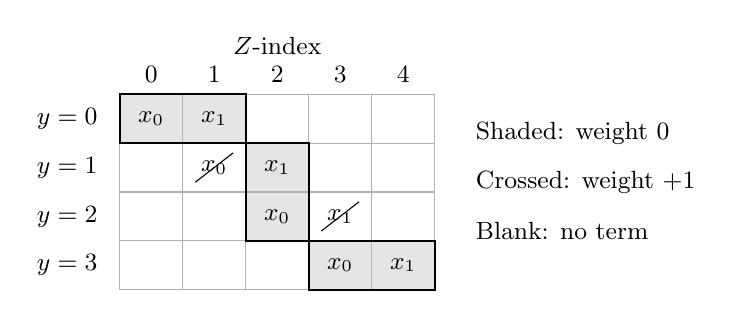
\begin{tikzpicture}[x=.8cm,y=.62cm,font=\small]
 \node at (2.5,5) {$Z$-index};
 \foreach \z in {0,...,4}{\node at (\z+.5,4.4) {$\z$};}
 \foreach \y in {0,...,3}{\node[anchor=east] at (-.2,3.5-\y) {$y=\y$};}
 \fill[gray!20] (0,3) rectangle (2,4);
 \fill[gray!20] (2,1) rectangle (3,3);
 \fill[gray!20] (3,0) rectangle (5,1);
 \draw[step=1,gray!60,thin] (0,0) grid (5,4);
 \draw[thick] (0,3) rectangle (2,4);
 \draw[thick] (2,1) rectangle (3,3);
 \draw[thick] (3,0) rectangle (5,1);
 \foreach \y in {0,...,3}{\foreach \i in {0,1}{
  \node at (\y+\i+.5,3.5-\y) {$x_{\i}$};}}
 \draw (1.2,2.2)--(1.8,2.8);
 \draw (3.2,1.2)--(3.8,1.8);
 \node[anchor=west] at (5.5,3.2) {Shaded: weight $0$};
 \node[anchor=west] at (5.5,2.2) {Crossed: weight $+1$};
 \node[anchor=west] at (5.5,1.2) {Blank: no term};
\end{tikzpicture}
\caption{The degeneration of $C(2,4)$, with $a=2,h=1$.
A cell $(y,z)$ contains $x_i$ when $z=y+i$. The three shaded
blocks survive, and the two crossed terms disappear. The blocks
have disjoint $Y$- and $Z$-coordinates but share $x_0,x_1$.
The middle block is $C(2,1)$ with its second and third legs exchanged
and its first-leg basis reversed.}
\label{fig:tripling}
\end{figure}

Translations identify the two outer branches with $C=C(a,h)$.
The middle branch is
\[
 \sum_{u=0}^{a-1}\sum_{r=0}^{h-1}
 x_{a-1-u}y_{h+u+r}z_{h+a-1+r}.
\]
It is $C$ with its second and third legs exchanged and its first-leg
basis reversed. The reversal identifies this individual branch;
no different first-leg maps are applied to the three branches of
the whole tensor.

Let $\sigma$ exchange the second and third legs. The uniform
probability vector on the three branches gives
\[
 \lambda_\pi(C(a,B))\geq
 3^{p_X^{(\pi)}}\lambda_\pi(C)^{2/3}
                       \lambda_\pi(C^\sigma)^{1/3}.
\]
Composition with $\sigma$ permutes the six leg permutations. Thus
$\prod_\pi\lambda_\pi(C^\sigma)=\prod_\pi\lambda_\pi(C)$.
Multiplying the six inequalities and taking the power $1/(6t)$
proves \eqref{eq:tripling}.
\end{proof}

\section{Discrete growth and the arithmetic exponent}\label{sec:growth}

The tensor constructions are complete. The following lemma turns the
profile's concavity and shifted tripling into growth along the diagonal.

\begin{lemma}[Diagonal growth]\label{lem:growth}
Let $P:\N_{>0}^2\to\R_{>0}$ be symmetric, with $P(1,b)=b$.
Suppose it satisfies \eqref{eq:concavity} for $a\geq1,b\geq2$ and
\eqref{eq:tripling} for $a,h\geq1$. Then
$P(a,a)\geq a^{4/3}$ for every $a\geq1$.
\end{lemma}

\begin{proof}
For fixed $a$, concavity makes the increments
$\Delta_{a,h}=P(a,h+1)-P(a,h)$ nonincreasing in $h$.
Set $D_a=P(a,a)$ and $H_a=2D_a/(3a-1)$. Tripling with $h=a$ gives
\[
 2D_a\leq P(a,4a-1)-D_a
       =\sum_{h=a}^{4a-2}\Delta_{a,h}
       \leq(3a-1)\Delta_{a,a}.
\]
Thus $\Delta_{a,a}\geq H_a$. For $a\geq2$, symmetry and concavity
bound the two increments between consecutive diagonal values:
\begin{equation}\label{eq:diagonal-rec}
 D_a-D_{a-1}
 =\Delta_{a-1,a-1}+\Delta_{a,a-1}
 \geq H_{a-1}+H_a.
\end{equation}
Substituting $D_a=(3a-1)H_a/2$, rearranging, and iterating from
$H_1=1$ gives
\begin{align}
 H_a&\geq\left(1+\frac1{3(a-1)}\right)H_{a-1}
          &&(a\geq2),\notag\\
 H_a&\geq\prod_{m=1}^{a-1}\left(1+\frac1{3m}\right)
          &&(a\geq1).\label{eq:normalized-growth}
\end{align}
For $a=1$ the product is empty and equals $1$.
For $m\geq1$, the elementary inequality
$(1+1/(3m))^3\geq1+1/m$ now gives
\[
 H_a^3\geq\prod_{m=1}^{a-1}\left(1+\frac1{3m}\right)^3
       \geq\prod_{m=1}^{a-1}\left(1+\frac1m\right)=a.
\]
Since $(3a-1)/2\geq a$, we conclude
$D_a\geq aH_a\geq a^{4/3}$.
\end{proof}

\begin{proof}[Proof of Theorem~\ref{thm:main}]
For every character, the profile \eqref{eq:profile} satisfies all
hypotheses of Lemma~\ref{lem:growth}. Combining it with
\eqref{eq:profile-basic} gives
\[
 a^{4/3}\leq P(a,a)\leq(2a-1)^{1/t}.
\]
Letting $a\to\infty$ forces $t\leq3/4$. Equation~\eqref{eq:character-mm}
therefore gives $\lambda(T_d)\leq d^{9/4}$ for every character.

For each integer $d\geq2$, take $k_d=\lceil d^\nu\rceil-1$.
Then $d^\nu-1\leq k_d<d^\nu$, so Lemma~\ref{lem:existence} supplies
a character with $\lambda(T_d)\geq k_d$. Hence
\[
 d^\nu\leq d^{9/4}+1.
\]
Taking logarithms and letting $d\to\infty$ yields $\nu\leq9/4$.
The detecting character may depend on $d$; the upper bound applies
uniformly to every character.

To obtain an arithmetic algorithm, fix $\eps>0$ and choose
$0<\delta<\eps$. The definition of $\nu$ supplies a fixed integer
$u\geq2$ and an exact rank decomposition of $T_u$ of length
$r<u^{9/4+\delta}$. Its bilinear identities remain valid on matrix
blocks: their coefficients are central scalars, and each product has
its left-input block before its right-input block.
For $N$ a power of $u$, recursive application therefore has cost
\[
 S(N)\leq rS(N/u)+C_{u,r}(N/u)^2.
\]
Flattening gives $r\geq u^2$. Summing the recursion levels gives
$S(N)=O(N^{\log_u r})$ if $r>u^2$, and
$S(N)=O(N^2\log N)$ if $r=u^2$. Both are
$O_\eps(N^{9/4+\eps})$. Padding an arbitrary $n$ to the next power
of $u$ increases its size by less than the fixed factor $u$ and
proves the theorem.
\end{proof}

\begin{remark}
All coefficients of the recursive algorithm are fixed once $\eps$ is
chosen. The argument is in the complex arithmetic model. If algebraic
coefficients are desired, the equations for an exact rank decomposition
have rational coefficients; a complex solution therefore implies a
solution over $\overline{\mathbb Q}$, by the Nullstellensatz.
The finitely many resulting coefficients lie in one number field.
\end{remark}

\appendix
\section{Existence of detecting characters}\label{sec:existence}

We prove Lemma~\ref{lem:existence} directly within the
asymptotic-spectrum framework~\cite{Str88,CVZ}.
A \emph{state} is a normalized, additive, restriction-monotone map
$S\to\R_{\geq0}$. Every state satisfies
$0\leq\lambda(s)\leq\rank(s)$, and $\lambda(s)\geq1$ for $s\ne0$.
A character is a state that is also multiplicative.

Fix integers $d\geq2$ and $k\geq0$ with $k<d^\nu$.
To obtain a character with $\lambda(T_d)\geq k$, we will construct
states satisfying the stronger family of inequalities
\begin{equation}\label{eq:detect-state}
 \lambda(T_ds)\geq k\lambda(s)\qquad(s\in S).
\end{equation}
This family is preserved by normalized tensor multiplication:
for any nonzero $z$, replacing $\lambda(x)$ by
$\lambda(zx)/\lambda(z)$ preserves every inequality by applying
\eqref{eq:detect-state} to $zs$.
The next lemma explains why this invariance produces multiplicativity
in a nonempty compact convex family of states.
We will then prove that the required family is nonempty. An empty
family would give tensors $D$ and $s\ne0$ with
$D+ks\geq D+T_ds$. Repeating this conversion while keeping $D$
fixed would contradict $k<d^\nu$.

\subsection{Obtaining multiplicativity}

\begin{lemma}\label{lem:multiplicativity}
Let $\mathcal K$ be a nonempty compact convex set of states in the
topology of coordinatewise convergence. Suppose that, for every
nonzero $z\in S$, the map
\[
 (P_z\lambda)(x)=\frac{\lambda(zx)}{\lambda(z)}
\]
takes $\mathcal K$ into itself. Then $\mathcal K$ contains a
multiplicative state.
\end{lemma}

\begin{proof}
Since $\lambda(z)\geq1$, each $P_z$ is continuous in the product
topology. The space $\R^S$ is Hausdorff and locally convex, so the
Schauder--Tychonoff fixed-point theorem~\cite{Tych35} applies: a
continuous self-map of a nonempty compact convex subset of such a
space has a fixed point. Choose a fixed point $\mu$ of $P_z$ and
freeze $c=\mu(z)$. The subset
\[
 \mathcal K'=
 \{\lambda\in\mathcal K:\lambda(zx)=c\lambda(x)
                  \text{ for every }x\in S\}
\]
is nonempty and compact. Because $c$ is fixed, its defining equations
are linear in $\lambda$, so it is convex. Taking $x=1$ shows that
$\lambda(z)=c$ throughout $\mathcal K'$, so all its members are
fixed by $P_z$. Moreover, every $P_w$ with $w\ne0$ preserves it:
\[
 (P_w\lambda)(zx)=\frac{\lambda(zwx)}{\lambda(w)}
                 =c\frac{\lambda(wx)}{\lambda(w)}
                 =c(P_w\lambda)(x).
\]
The construction can be repeated in $\mathcal K'$, retaining all
earlier frozen equations. By induction, every finite collection of
the original maps $P_z$ has a common fixed point in $\mathcal K$.
Their fixed sets are closed, so compactness and the finite
intersection property give a simultaneous fixed point for all
nonzero $z$. It satisfies
$\lambda(zx)=\lambda(z)\lambda(x)$ for $z\ne0$. Additivity implies
$\lambda(0)=0$, which handles multiplication by zero.
\end{proof}

\subsection{Constructing the detecting state space}

\begin{proof}[Proof of Lemma~\ref{lem:existence}]
For the fixed integers $d,k$ above, let $\mathcal K$ be the subset of
$\prod_{s\in S}[0,\rank(s)]$ defined by normalization, additivity,
monotonicity, and \eqref{eq:detect-state}. These conditions are closed affine equalities and inequalities. The product is compact, so $\mathcal K$ is compact and
convex. We must first show that it is nonempty.

Suppose it were empty. Compactness supplies a finite inconsistent
subsystem of the defining conditions. Let $E\subset S$ contain every
coordinate appearing in this subsystem, together with $0$ and $1$.
Adjoin $\lambda(0)=0$, $\lambda(1)=1$, and write each coordinate bound
homogeneously as
\[
 \lambda(s)\geq0,\qquad
 \rank(s)\lambda(1)-\lambda(s)\geq0\quad(s\in E).
\]
The resulting finite system remains inconsistent.

Let $e_s$, $s\in E$, be the coordinate vectors of $\R^E$.
Quotient by the span of the selected additive relation vectors and
$e_0$, and write $u$ for the image of $e_1$. Let $C$ be the cone
generated by the images of all inequality vectors. Before taking the
quotient, these vectors have the forms
\[
 e_b-e_a\ (b\geq a),\qquad e_{T_ds}-ke_s,\qquad
 e_s,\qquad \rank(s)e_1-e_s.
\]
The finitely generated cone $C$ is closed. If $-u\notin C$, separation
gives a linear functional $L$ nonnegative on $C$ with $L(u)>0$.
Dividing by $L(u)$ would give a normalized solution of the finite
subsystem, including its bounds. This contradicts inconsistency, so
$-u\in C$.

All vectors and relations have integer coefficients. Membership
$-u\in C$ is a feasible rational linear system, so there are rational
nonnegative cone coefficients and rational coefficients for the
relation vectors. Clearing denominators yields a positive integer
$m$ and an identity with nonnegative integer coefficients on the
inequality vectors.

Map this identity to the additive Grothendieck group of $S$ by sending
$e_s$ to $[s]$. This group adjoins formal additive inverses to the
commutative monoid $(S,+)$; in particular, all additive relation
vectors map to zero. The bound vectors map to the order differences
$[s]-[0]$ and $[\rank(s)]-[s]$. Direct sums combine the ordinary order
differences into $[y]-[x]$ with $y\geq x$. Distributivity combines the
special differences into $[T_ds]-k[s]$ for one $s\in S$. We obtain
\[
 -m[1]=[y]-[x]+[T_ds]-k[s],\qquad y\geq x.
\]
Equality in this group means equality after adding a common element
of the monoid. Thus there is $c\in S$ with
\[
 m+y+T_ds+c=x+ks+c.
\]
Put $D=y+c$. Using $y\geq x$ gives the catalytic comparison
\begin{equation}\label{eq:catalyst}
 D+ks\geq D+m+T_ds.
\end{equation}
Here $s\ne0$: otherwise $D\geq D+m$, contradicting the additivity
and monotonicity of any flattening rank.

\medskip
\noindent\emph{Ruling out the obstruction.}
The tensor $D$ is a fixed additive cost. Reusing
\eqref{eq:catalyst} converts $nk$ copies of $s$ into $n$ copies of
$T_ds$ while paying for $D$ only once. We show that this contradicts
the definition of $\nu$. Additive iteration gives, for every integer $n\geq1$,
\[
 D+nks\geq D+nm+nT_ds\geq nT_ds.
\]
Since $s\geq1$, we have $\rank(D)s\geq\rank(D)\geq D$.
With $K=nk+\rank(D)$, it follows that
\begin{equation}\label{eq:amplification}
 Ks\geq nT_ds,\qquad K^js\geq n^jT_{d^j}s\quad(j\geq1).
\end{equation}
For the induction, multiply the $j$th comparison by $K$, then use
$Ks\geq nT_ds$:
\[
 K^{j+1}s\geq n^jT_d^j(Ks)\geq n^{j+1}T_d^{j+1}s.
\]
This keeps a single factor $s$ and requires no cancellation.
Also $K>0$, since the first right-hand side in
\eqref{eq:amplification} is nonzero.

We next use the $n^j$ scalar copies to obtain a second
matrix-multiplication factor. Its matrix dimension will multiply
$d^j$, while the auxiliary tensor $s$ still occurs only once.
Fix $n$ and $\delta>0$. By the definition of $\nu$, choose a fixed
integer $u\geq2$ with $\rank(T_u)\leq u^{\nu+\delta}$, and set
\[
 \ell_j=\left\lfloor\frac{j\log_u n}{\nu+\delta}\right\rfloor,
 \qquad g_j=u^{\ell_j}.
\]
Submultiplicativity gives
\[
 \rank(T_{g_j})\leq\rank(T_u)^{\ell_j}
 \leq u^{(\nu+\delta)\ell_j}\leq n^j.
\]
Thus the diagonal tensor $n^j$ restricts to $T_{g_j}$. Multiplying
this restriction by $T_{d^j}s$ and using $s\geq1$, we obtain
\[
 K^js\geq n^jT_{d^j}s\geq T_{d^jg_j}s\geq T_{d^jg_j}.
\]
A direct sum of $K^j$ copies of $s$ has rank at most $K^j\rank(s)$.
Therefore
\[
 \rank(s)K^j\geq\rank(T_{d^jg_j})\geq(d^jg_j)^\nu.
\]
First let $j\to\infty$, keeping $n,\delta,u$ fixed. Since
$g_j^{1/j}\to n^{1/(\nu+\delta)}$, taking $j$th roots gives
\[
 nk+\rank(D)\geq d^\nu n^{\nu/(\nu+\delta)}.
\]
Next let $\delta\downarrow0$ at fixed $n$; the choice of $u$ has
disappeared from the inequality. We get
$nk+\rank(D)\geq nd^\nu$. Finally divide by $n$ and let
$n\to\infty$. The catalyst $D$ is fixed, so $k\geq d^\nu$,
a contradiction. Consequently $\mathcal K$ is nonempty.

\medskip
\noindent\emph{Completing the construction.}
For nonzero $z$, the map $P_z$ of Lemma~\ref{lem:multiplicativity}
preserves normalization, additivity, and monotonicity. It preserves
\eqref{eq:detect-state}, because
\[
 (P_z\lambda)(T_ds)=\frac{\lambda(T_dzs)}{\lambda(z)}
 \geq k\frac{\lambda(zs)}{\lambda(z)}=k(P_z\lambda)(s).
\]
Its coordinate bounds follow from $zx\leq\rank(x)z$.
Lemma~\ref{lem:multiplicativity} supplies a multiplicative state in
$\mathcal K$, hence a character. Taking $s=1$ in
\eqref{eq:detect-state} gives $\lambda(T_d)\geq k$.
\end{proof}

\begin{thebibliography}{99}

\bibitem{AD25}
J. Alman, R. Duan, V. Vassilevska Williams, Y. Xu, Z. Xu, and R. Zhou,
More asymmetry yields faster matrix multiplication,
in \emph{Proc. 2025 Annual ACM-SIAM Symposium on Discrete Algorithms},
SIAM, 2025, 2005--2039.
\href{https://doi.org/10.1137/1.9781611978322.63}{doi:10.1137/1.9781611978322.63}.

\bibitem{AW21}
J. Alman and V. Vassilevska Williams, A refined laser method and faster
matrix multiplication, \emph{TheoretiCS} \textbf{3} (2024), Article 21, 1--32.
\href{https://doi.org/10.46298/theoretics.24.21}{doi:10.46298/theoretics.24.21}.
Conference version in SODA 2021, 522--539.

\bibitem{Bini80}
D. Bini, Relations between exact and approximate bilinear algorithms.
Applications, \emph{Calcolo} \textbf{17} (1980), 87--97.
\href{https://doi.org/10.1007/BF02575865}{doi:10.1007/BF02575865}.

\bibitem{CVZ}
M. Christandl, P. Vrana, and J. Zuiddam, Universal points in the
asymptotic spectrum of tensors, \emph{J. Amer. Math. Soc.}
\textbf{36} (2023), 31--79.
\href{https://doi.org/10.1090/jams/996}{doi:10.1090/jams/996}.

\bibitem{CW90}
D. Coppersmith and S. Winograd, Matrix multiplication via arithmetic
progressions, \emph{J. Symbolic Comput.} \textbf{9} (1990), 251--280.
\href{https://doi.org/10.1016/S0747-7171(08)80013-2}{doi:10.1016/S0747-7171(08)80013-2}.

\bibitem{DS13}
A. M. Davie and A. J. Stothers, Improved bound for complexity of
matrix multiplication, \emph{Proc. Roy. Soc. Edinburgh Sect. A}
\textbf{143} (2013), 351--369.
\href{https://doi.org/10.1017/S0308210511001648}{doi:10.1017/S0308210511001648}.

\bibitem{DWZ23}
R. Duan, H. Wu, and R. Zhou, Faster matrix multiplication via asymmetric
hashing, in \emph{Proc. 64th IEEE Annual Symposium on Foundations of
Computer Science}, IEEE, 2023, 2129--2138.
\href{https://doi.org/10.1109/FOCS57990.2023.00130}{doi:10.1109/FOCS57990.2023.00130}.

\bibitem{Dup26}
E. Dupont, M. Eisenberger, B. Kozlovskii, A. Mehrabian, F. J. R. Ruiz,
A. See, R. Zhou, J. Alman, V. Vassilevska Williams, and M. Balog,
Improving the matrix multiplication exponent with modern optimization
and AlphaEvolve, preprint, 2026.
\href{https://arxiv.org/abs/2608.16884}{arXiv:2608.16884}.

\bibitem{Kow14}
E. Kowalski, \emph{An introduction to the representation theory of groups},
Graduate Studies in Mathematics \textbf{155}, American Mathematical
Society, 2014.
\href{https://doi.org/10.1090/gsm/155}{doi:10.1090/gsm/155}.
Author version: \emph{Representation theory}, February 17, 2017,
\href{https://people.math.ethz.ch/~kowalski/representation-theory.pdf}{Section~2.6}.

\bibitem{LG14}
F. Le Gall, Powers of tensors and fast matrix multiplication,
in \emph{Proc. 39th International Symposium on Symbolic and Algebraic
Computation}, ACM, 2014, 296--303.
Full version: \href{https://arxiv.org/abs/1401.7714v1}{arXiv:1401.7714v1}.

\bibitem{Sch81}
A. Sch\"onhage, Partial and total matrix multiplication,
\emph{SIAM J. Comput.} \textbf{10} (1981), 434--455.
\href{https://doi.org/10.1137/0210032}{doi:10.1137/0210032}.

\bibitem{Sto10}
A. J. Stothers, \emph{On the complexity of matrix multiplication},
Ph.D. thesis, University of Edinburgh, 2010.
\href{https://hdl.handle.net/1842/4734}{hdl:1842/4734}.

\bibitem{Str69}
V. Strassen, Gaussian elimination is not optimal,
\emph{Numer. Math.} \textbf{13} (1969), 354--356.
\href{https://doi.org/10.1007/BF02165411}{doi:10.1007/BF02165411}.

\bibitem{Str86}
V. Strassen, The asymptotic spectrum of tensors and the exponent of
matrix multiplication, in \emph{Proc. 27th Annual Symposium on
Foundations of Computer Science}, IEEE, 1986, 49--54.
\href{https://doi.org/10.1109/SFCS.1986.52}{doi:10.1109/SFCS.1986.52}.

\bibitem{Str87}
V. Strassen, Relative bilinear complexity and matrix multiplication,
\emph{J. Reine Angew. Math.} \textbf{375/376} (1987), 406--443.
\href{https://doi.org/10.1515/crll.1987.375-376.406}{doi:10.1515/crll.1987.375-376.406}.

\bibitem{Str88}
V. Strassen, The asymptotic spectrum of tensors,
\emph{J. Reine Angew. Math.} \textbf{384} (1988), 102--152.
\href{https://doi.org/10.1515/crll.1988.384.102}{doi:10.1515/crll.1988.384.102}.

\bibitem{Tych35}
A. Tychonoff, Ein Fixpunktsatz,
\emph{Math. Ann.} \textbf{111} (1935), 767--776.
\href{https://doi.org/10.1007/BF01472256}{doi:10.1007/BF01472256}.

\bibitem{VW12}
V. Vassilevska Williams, Multiplying matrices faster than
Coppersmith--Winograd, in \emph{Proc. 44th Annual ACM Symposium
on Theory of Computing}, ACM, 2012, 887--898.
\href{https://doi.org/10.1145/2213977.2214056}{doi:10.1145/2213977.2214056}.
Expanded corrected author version: \emph{Multiplying matrices in
$O(n^{2.373})$ time}, July 1, 2014.

\bibitem{VXXZ24}
V. Vassilevska Williams, Y. Xu, Z. Xu, and R. Zhou,
New bounds for matrix multiplication: from alpha to omega,
in \emph{Proc. 2024 Annual ACM-SIAM Symposium on Discrete Algorithms},
SIAM, 2024, 3792--3835.
\href{https://doi.org/10.1137/1.9781611977912.134}{doi:10.1137/1.9781611977912.134}.

\end{thebibliography}
\end{document}
